%!TEX root = ../../thirdYearReport.tex


\paragraph{Work package 4 progress}

\subparagraph*{Improved Models from Real-Time Regression with Latent Contact Type Inference (T4.1)}

%!TEX root = ../../thirdYearReport.tex


Within T4.1 IIT developed a theoretical framework for estimating whole-body
dynamics from distributed multimodal sensors \cite{Nori2015}. Considered sensors
include joint encoders, gyroscopes, accelerometers and force/torque sensors.
Estimated quantities are position, velocity, acceleration and (internal and
external) wrenches on all the rigid bodies composing the robot articulated
chain. The estimation procedure consists of an extended Kalman filter (EKF)
which gives the a-posteriori estimation given all the available measurements.
Computational efficiency is obtained by formulating the Kalman filter
update-step with a sparse Bayesian network. Experiments for validating the
proposed theoretical framework have been conducted on a leg of the iCub humanoid
robot. The iCub is an ideal platform for the proposed experiment given its
distributed force, torque, linear acceleration and angular velocity sensors.
Results have shown the accuracy and the computational efficiency of the proposed
method. The theoretical framework has been implemented in an open source
software (see also Section \ref{sec:T15}).

\subparagraph*{Inferring the Operational Space and Appropriate Controls with Multiple Contacts (T4.2) (TUD: 6PM)}%(TUD 4PM, ??PARTNERS)}

%TUD

%Elmar 
During year two, TUD and JSI investigated the effect of supportive contacts on 
postural control. First results were presented during the second year review 
meeting (Task T2.4 on Human contact choice and learning through physical 
interaction). During year three, we collected a large dataset of more than 
$9.000$ reaching movements in $20$ subjects. To analyze the data TUD developed a 
probabilistic model which extends classical statistical tests (ANOVA test of 
contact locations and target locations, movement onsets, etc.). The 
probabilistic model allows for detailed investigations of movement kinematics in 
a spaciotemporal domain and extends classical techniques that rely on scalar 
descriptors of the complex motion patterns. In whole body adaptation 
experiments, shown in Figure \ref{fig:subFigContactLocationsAllSubjects}, TUD 
and JSI found strong correlations between both arms and the trunk. These 
correlations were used to predict the reaching motion from early phase 
observations of the supportive contact motion. The results suggest that postural 
control predicts and precedes goal-directed movements, which has the potential 
to impact pre-tests of central nervous system disorders like dementia, 
Alzheimer's or Parkinson's disease that are less prone to factors like stress, 
sleep deprivation and age compared to the classical cognitive tests. A pre-print 
of a paper that was submitted for review to Scientific Reports is given in 
Deliverable D2.2.

\begin{figure}%[t]
\centering
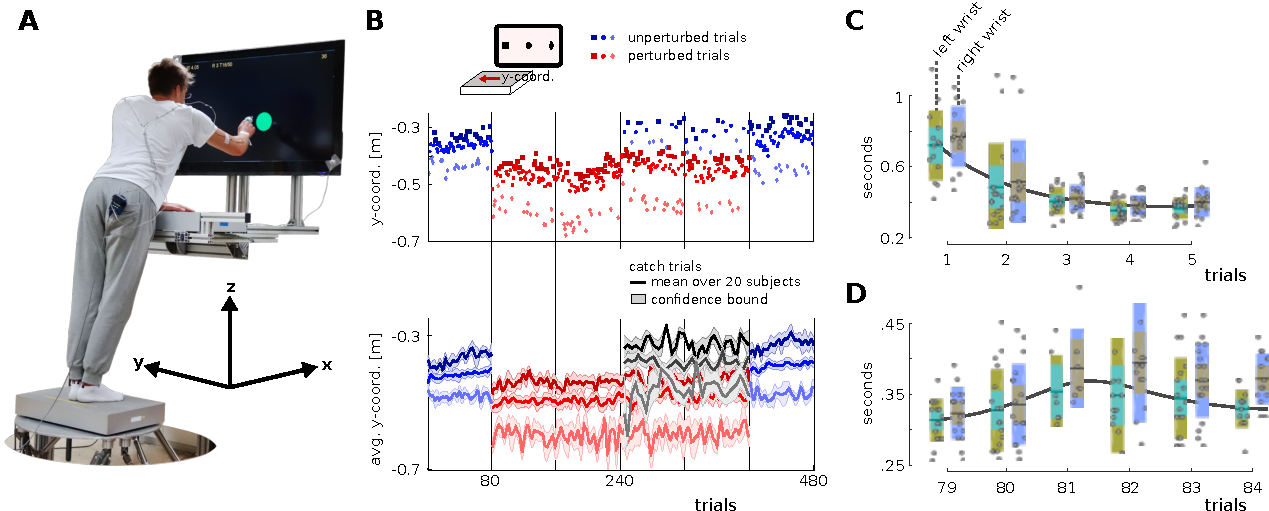
\includegraphics[width=\textwidth]{images/Figure-1(rueckert)}
%\label{fig:subfig2}
 \caption[Human reaching experiment with target dependent contacts and synchronized arm motions.]{\textbf{Experiment, target dependent contacts and synchronized arm motions.} \textbf{A)} Experimental setting. 
 \textbf{B)}  The top row shows contact locations for a single representative subject 
 and the bottom row shows the mean and the confidence bound over all $20$ participants. 
 The first $80$ trials and the last $80$ trials are unperturbed sessions. 
 Catch trials were initiated during trials $240$ to $400$ and are denoted by the black lines in \textbf{B}.
 \textbf{C)} Illustration of the movement onsets of the wrists for the first five trials. 
 \textbf{D)} Movement onsets for the first six trials transitioning to the perturbed session. 
}
\label{fig:subFigContactLocationsAllSubjects}
\end{figure}

In ongoing work, TUD and JSI investigate how such probabilistic models can predict when 
and how to make supportive contacts in robot reaching tasks. Our goal is to 
reproduce the correlated reaching and supportive contact motions in the ICub robot. 
In addition to the target dependent contact locations, a module that predicts 
when to initiate a supportive contact will be developed. This model will make 
use of the estimated center of pressure using the two force/torque sensors in the 
ankles. 

\begin{figure}
\centering
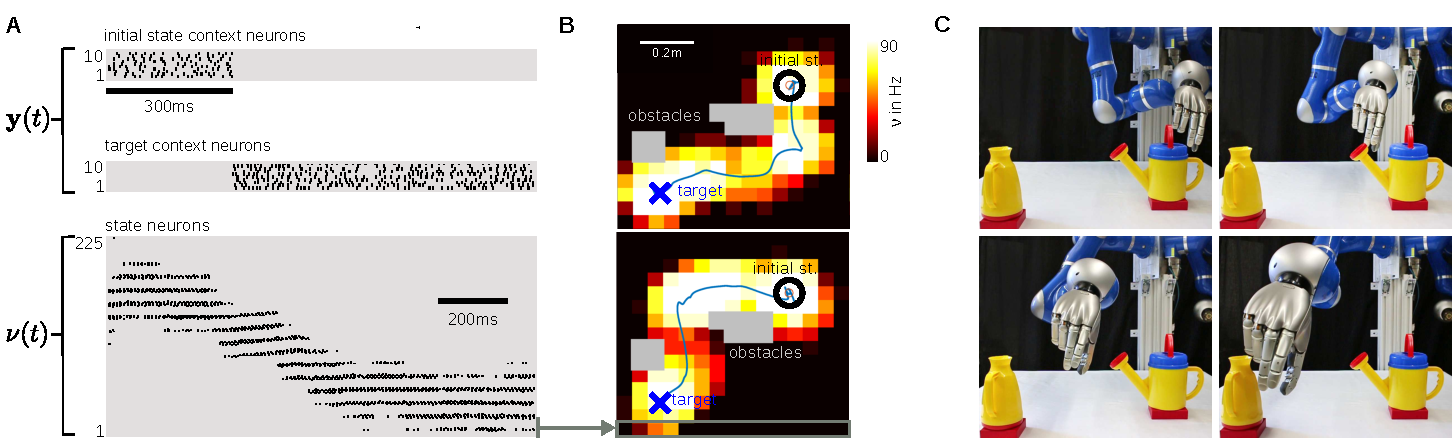
\includegraphics[width=\textwidth]{images/KukaLearnedModelObstacles}
%\label{fig:subfig2}
 \caption[Planning in spkining neural networks with multiple constraints on a Kuka robot.]{\textbf{Planning with multiple constraints on a real robot.} {\bf A)} Generated 
spike train (top: context neurons, bottom: state neurons) after contrastive 
divergence learning of the transition model. {\bf B)} Two sampled movement plans 
solving the obstacle avoidance task. {\bf C)} Snapshots of the executed movement 
on the real robot.
}
\label{fig:exp_kukaRueckert}
\end{figure}

In another approach, TUD investigated computational models of operational space 
control in rodents using spiking neural networks. While this study is more of a 
fundamental type and does not directly provide concrete algorithms for humanoid 
robot control, it has interesting potentials for the challenging tasks in 
CoDyCo. Concretely, in spiking neural networks arbitrary-shaped obstacles can be 
modeled, non-linearities in the transition model due to contacts can be learned 
and movement plans can computed much faster then real-time through exploiting 
local-only dependencies. These advantages were evaluated in target-reaching task 
in a Kuka robot arm. For that TUD developed learning algorithms grounded in the 
theory of probabilistic inference to train the recurrent spiking neural network 
from human demonstrations. The training data was collected in kinesthetic 
teaching. After the training, the network model was used to plan goal-directed 
task space trajectories that avoid obstacles in the three-dimensional space. Two 
example movements and the corresponding neural activity are illustrated in 
Figure \ref{fig:exp_kukaRueckert}. For details on the approach we refer to 
Deliverable D4.1. A manuscript on this work was accepted for publication in 
Scientific Reports~\cite{Rueckert_SR_2016} (impact factor 5.578 in 2014). 

In a student's master thesis, TUD extended the model to jointly model 
configuration and task spaces. This extension is based on factorized population 
codes and allows for applications to high-dimensional robot systems. In ongoing 
work, TUD will test the learning algorithms of the spiking network in the ICub 
robot.    


\subparagraph*{Learning the Prioritization of Tasks (T4.4) (TUD: 6PM, UPMC: 0.74)}%(TUD 3.2PM, INRIA 2PM)}

During the third year, TUD continued its research on learning controllers for 
physical interaction. We presented a novel approach at an international robotics 
conference~\cite{paraschos2015model}. The approach learns and generates 
movements for physical interaction that are trained with imitation learning from 
a small set of demonstrated trajectories. Learning such a model is a non-trivial 
task and therefore we introduced the \textit{model-free} Probabilistic Movement 
Primitives (ProMPs). Here, we learn jointly the movement and the necessary 
actions from a few demonstrations. We derived a variable stiffness controller 
analytically and we extended the ProMPs to include force and torque signals, 
necessary for physical interaction in the CoDyCo scenarios. 

Based on these results we also focused on developing a novel approach for task 
prioritization during year three. Our approach follows the concept of ``soft'' 
priorities, where a task which is lower in the task-hierarchy can controllably 
interfere with a higher-priority task. This concept is applicable to a wide-set 
of problems including balancing and reaching in humanoids with physical contacts 
with the environment. In our approach we dynamically change the priority of each 
task in time and, thus, adapt the behavior of the robot dynamically.  The 
approach utilizes imitation learning to obtain the variance of each task 
movement which is then used as the relative priority of the task. An important 
contribution of our approach shows how we can utilize probabilistic methods to 
analytically derive the tasks priorities from the imitation learning. We relate 
our approach to other state-of-the-art movement prioritization 
approaches~\cite{Peters_AR_2008, lober2015variance} and we show how these 
approaches can be derived under our framework. We provide an alternative point 
of view on movement prioritization that is derived from first-order principles. 
We demonstrated that our approach achieves improved performance and that is 
numerically stable, avoiding singularities. A paper on this approach was 
submitted to a robotics conference.

The at UPMC developed whole-body controllers allow multiple concurrent tasks to be 
executed on redundant robots, and such combinations often engender unforeseeable 
incompatibilities between the tasks due to conflicting task objectives and the 
robot's constraints. The result is typically a failure of one or more tasks to 
be properly carried out. In \cite{lober-HUMANOIDS2014}, UPMC introduced a measure of task 
compatibility, or compatibility cost. By optimizing parametric task 
representations, UPMC was able to minimize said cost and render the tasks 
compatible, albeit slowly. In \cite{lober2015variance}, UPMC looked at how task 
priorities could be automatically modulated by the variance associated with each 
task. This provided a reactive way to handle many common incompatibility 
scenarios. Currently, lately UPMC has been working on more computationally 
efficient task compatibility optimization schemes which combine the previous two 
works.   
